\chapter{Evaluation}
\label{sec:eval}
This section covers the evaluation of the proposed thesis. We will
evaluate the robot memory qualitatively in both application domains,
the RCLL and RoboCup@Home league, and quantitatively.

The qualitative evaluation analyzes how well the robot memory can be
used, how useful it is, and where difficulties are. It also includes
analyzing the expressiveness and convenience of representing and
querying knowledge, the integration into KBS
languages, and the shared access to the robot memory across different
applications and robots. To perform the qualitative evaluation, we
will implement prototypes using main features of the robot
memory. These prototypes act as proof of concept without implementing
complete domain solutions which would extend the scope of the thesis.
%
The general storage and query features of the robot memory will be
evaluated in the RCLL context with a CLIPS agent that stores the world
model in the robot memory and keeps it up to date. This shows how well
the robot memory can be integrated in a reasoner.
%
In a second step, the world model should be synchronized between a
multi-robot team to evaluate how well the shared robot memory works in
a distributed system. This includes an analysis of the network
throughput and robustness to package loss.
%
The planner specific view of the robot memory will be evaluated with a
PDDL planner in the RCLL domain. The robot-memory-PDDL interface
should generate a PDDL problem description from a world model stored
in the robot memory. The resulting plan should be stored in the robot
memory and queryable by CLIPS.
%
To evaluate event-triggers, we will register events depending on
changes of the RCLL world model that need to be updated in the local
CLIPS agent. Furthermore we want to try more complex events, which
could be used to trigger actions in the @Home domain (e.g. the space
occupied by objects in the dishwasher is high enough to start it).
This should show how useful and expressive registered events can be.
% 
These prototypes should show if the robot memory allows knowledge
sharing between multiple KBS. A related thesis,
which is in preparation, wants to utilize PDDL for global task
planning and CLIPS for execution to achieve more efficient multi-robot
behavior in the RCLL. It could benefit from using the robot memory and
yield further evaluation results.

To further evaluate how well the robot memory works in a hybrid
reasoning context with motion planners and symbolic planners, we will
also develop a RoboCup@Home related prototype using computables. Here
the robot memory should hold knowledge usable by a motion planner and
transform it into symbolic knowledge usable by a reasoner (e.g. if the
robot's coordinates are stored and a reasoner asks for the room the
robot is in). Thus a computable has to compute the symbolic knowledge
from the spatio-temporal one or vice versa. Quantitatively,
computables have to be evaluated by comparing the times between giving
the query and receiving the results with and without computables
taking the computation time, either on demand or on changing data.

To analyze how the query computation time increases with increasing query
expressiveness and database scale, we want to implement a simple
tidying up scenario. The robot memory models a scene with current
object placements and object storage positions in increasing
amount. The queries start simple (e.g. where is the storage place for
the red cup) and get more complex (e.g. which objects are not at their
storage position). Furthermore, the CPU and memory usage of the robot
memory have to be analyzed as well as the size of the database on the
hard drive.


\section{Schedule}
\begin{table}
  \centering
  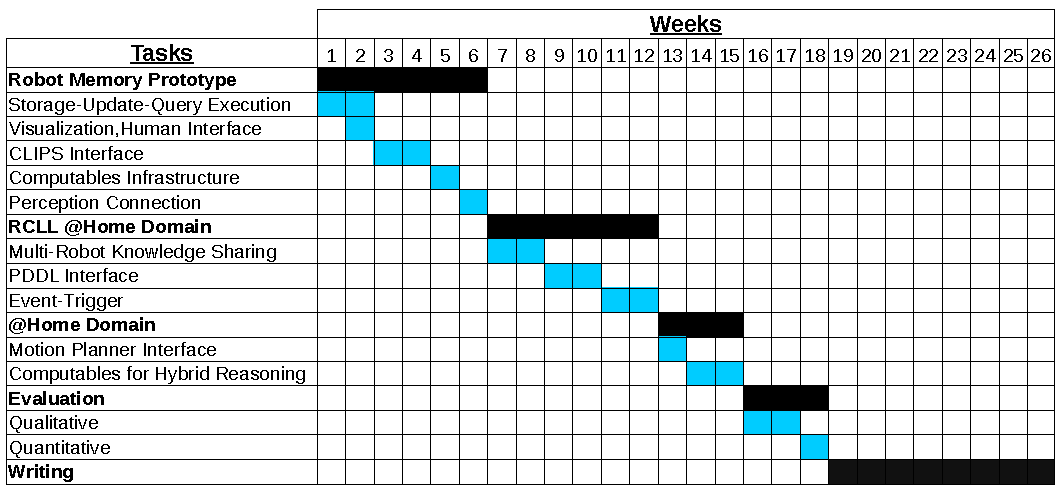
\includegraphics[width=\textwidth]{gantt-chart}%
  \vspace{-5mm}
  \caption{Gantt Chart of the thesis time schedule}
  \label{tab:gantt}
\end{table}
The time-schedule of the thesis is shown in \reftab{tab:gantt}. The
first part focuses on developing a robot-memory prototype with the
CLIPS interface, infrastructure for computables, and fundamental
connection to perception components. This prototype is then
iteratively improved to implement all other features needed in the
RCLL and in RoboCup@Home domain. The robot-memory itself and both
applications are then evaluated and the rest of the time is spent on
the written report.
